%! Author = Justus Benedict Siegert
%! Date = 22.01.2023

% Preamble
\documentclass[a4paper,10pt]{scrartcl}

\bibliographystyle{plain}

% Packages
\usepackage[utf8]{inputenc}
\usepackage[ngerman]{babel}
\usepackage[T1]{fontenc}
\usepackage[normalem]{ulem}
\usepackage{wasysym}
\usepackage{graphicx}
\useunder{\uline}{\ul}{}


% Document
\begin{document}
    \title{Lucky Thirteen}
    \author{Justus Benedict Siegert}
    \date{8445024, s222312@student.dhbw-mannheim.de}
    \maketitle
    \tableofcontents
    \newpage


    \section{Einleitung}\label{sec:einleitung}
    Das Verschlüsseln von Daten ist seit der Nutzung des Internets ein wichtiges Anliegen der Nutzenden.
    Ein viel genutzte Protokoll ist das Transport Layer Security Protokoll (TLS)\cite{letcencrypt2023}.
    Lucky 13 ist eine kryptografische Schwachstelle des TLS-Protokolls in den Versionen 1.0 und 1.1, sowie in Secure Socket Layer (SSL) und im Datagram Transport Layer Security (DTLS).
    Dabei müssen diese Versionen der Protokolle Maßnahmen gegen eine Padding Oracle Attack enthalten~\cite[S.2]{AlFardan2013}.
    Falls dies nicht der Fall ist, sind andere Angriffe möglich.
    Durch die Schwachstelle können Angreifer Daten ausspionieren, die verschlüsselt und vermeintlich sicher sind.
    Die Sicherheitslücke wurde 2013 von den Wissenschaftlern Nadhem J. AlFardan and Kenneth G. Paterson der Security Group der Royal Holloway University of London entdeckt.
    \newline
    Der Lucky 13 Angriff ist eine Art von Man-in-the-Middle-Attack, verbunden mit einer Padding Oracle Attack.
    Dies ist notwendig, weil sich der Angreifer zwischen Client und Server befinden muss, um die verschlüsselten Nachrichten lesen und senden zu können.
    Gleichzeitig beruht der Angriff auf einer Padding Oracle Attack, wo verschiedene Paddings an einen Server geschickt werden, um das richtig formatierte zu erfahren.
    Dabei ist das Problem, dass das Padding nach der Berechnung des Message Authentication Code (MAC) hinzugefügt wird und somit unauthentifizierte Daten im verschlüsselten Klartext bildet\cite[S.2]{AlFardan2013}. %Quelle
    Im Folgendem werden verschiedene Aspekte zum Verständnis der Sicherheitslücke ausgeführt.

    \subsection{Man-in-the-Middle-Attack}\label{subsec:man-in-the-middle-attack}
    Eine Man-in-the-Middle-Attack (MITM) ist ein Angriff, bei dem eine dritte Partei eine vermeintlich direkte sichere Verbindung von zwei anderen zwischen geschaltet ist.
    Bei einem solchen Angriff wird unerlaubt auf den Datenverkehr zweier Kommunikationspartner zugegriffen, in dem der Angreifer versucht zwischen den Datenverkehr der beiden Kommunikationspartner zu gelangen und diesen abzufangen oder zu manipulieren.
    Die Gefahr dabei ist, dass es nicht im Rahmen einer normalen Datenübertragung zu erkennen ist, ob jemand sich dazwischen geschaltet hat.
    %eleg unsichere aussage

    \subsection{Padding Oracle Attack}\label{subsec:padding-oracle-attack}
    Die Padding Oracle Attack wurde 2002 von Vaudenay entdeckt und dient als Basis für diesen Angriff.
    Bei einer Padding Oracle Attack wird ausgenutzt, dass einige Chiffren ein Padding benötigen, um eine Nachricht auf die benötigte Blocklänge zu verlängern, damit eine Blockverschlüsslung durchführbar ist~\cite[S.1]{Vaudenay2002}.
    Der Angreifer schickt dann Nachrichten an den Server mit verschiedenen Paddings und schaut, ob der Server diese akzeptiert.
    Bei einem korrektem Padding kann dann die Nachricht genutzt werden, um die Verschlüsslung der Datenpakete zu brechen.
    Durch die präzise Antwort des Servers, dass es zu einem Entschlüsselungsfehler und keinen Paddingfehler kam, resultiert der Name Oracle\cite{Rizzo2010}.
    Um einen gewöhnlichen Angriff zu verhindern, wurden die Server so konfiguriert, dass nur eine allgemein eine Fehlerrückmeldung gesendet wird, die nicht auf die Art des Fehlers schließen lässt~\cite[S.6]{Vaudenay2002}.
    \newline
    Bei dem Beispiel im Paper von Nadhem J. AlFardan and Kenneth G. Paterson wurde lediglich der Angriff in Verbindung mit der Blockchiffre Cipher Block Chaining (CBC) verwendet.
    Dies ist ein Beispiel für einen Verschlüsselungsalgorithmus, bei dem der Angriff möglich ist \cite{Vaudenay2002}.


    \section{(Datagram) Transport Layer Security}\label{sec:(d)tls}
    Der Vorgänger von TLS, Secure Socket Layer (SSL) 1.0 erschien im Jahr 1994, neun Monate nach der ersten Mosaic Version~\cite{Schwenk2022}.
    In den folgenden zwei Jahre wurden zwei weiter Versionen entwickelt und dann SSL in TLS 1.0 umbenannt.
    \newline
    TLS besteht aus zwei Hauptkomponenten: dem TLS Handshake, der für den sicheren Schlüsselaustausch zwischen dem Client und dem Server zuständig ist,
    und dem TLS Record.
    Dieser verwendet die beim Handshake ausgehandelten Schlüssel, um eine sichere Datenübertragung zu ermöglichen.
    Die Daten werden verschlüsselt und mit einem MAC gegen Manipulation geschützt.
    Die grundlegende Funktionsweise besteht darin, dass der Client eine Verbindung mit dem Server aufbaut, welcher sich mit einem Zertifikat authentifiziert.
    Der Client überprüft die Vertrauenswürdigkeit durch einen Vergleich der Daten des Zertifikats mit denen des Servers.
    \newline
    DTLS basiert auf TLS, kann aber im Gegensatz zu TLS auch Transportprotokolle wie User Datagram Protocol (UDP) übertragen.
    Es hat aber grundlegend dieselben Eigenschaften und Sicherheitsmerkmale.

    \subsection{Cipher Block Chaining Mode}\label{subsec:cbc-mode}
    Cipher Block Chaining Mode (CBC) ist eine Variation, die bei Blockchiffre genutzt werden kann.
    Dabei wird der Klartextblock vor dem Verschlüsseln mit dem vorherigen verschlüsselten Block per XOR verknüpft\ref{CBC_Mode}.
    Die Vorteile dieses Modus sind, dass gleiche Klartextblöcke unterschiedlich verschlüsselte Blöcke ergeben.
    Der Nachteil besteht allerdings darin, dass nicht gleichzeitig mehrere Blöcke verschlüsselt werden können, da diese voneinander abhängen.
    Der weitere Verlauf wird unter der Annahme des CBC-Modes beschrieben.
    \begin{figure}[h]
        \begin{center}
            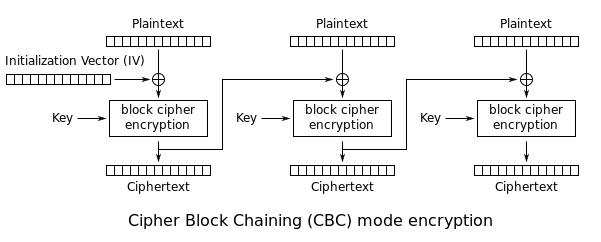
\includegraphics[width=12cm]{./Literatur/documents/wo8Bl}\newline\caption{Verschlüsselung im CBC-Mode~\cite{CBC-verschluesseln}}
            \label{CBC_Mode}
        \end{center}
    \end{figure}


    \section{Voraussetzungen für einen Angriff}\label{sec:voraussetzungen-fur-einen-angriff}
    Damit ein Lucky 13 Angriff gelingt, muss auf der Serverseite die TLS Version 1.1 oder älter mit Maßnahmen gegen den Padding Oracle Attack laufen.
    Der Angriff ist darauf ausgelegt die Maßnahmen gegen einen normale Padding Oracle Attack zu umgehen, indem die Padding-Überprüfung beim Server nicht über den Inhalt der Antwort analysiert wird, sondern über die Verarbeitungszeit.
    Bei anderen, älteren Versionen ist der Angriff deshalb nicht empfehlenswert, weil es andere, einfachere Sicherheitslücken zum Ausnutzen gibt.
    \newline
    Lucky 13 nutzt den Zeitkanal aus, welcher nur im lokalen Netzwerk des Servers getestet wurde.
    Um eine genaue Zeitmessung zu ermöglichen, muss man das Rauschen des Netzwerks analysieren, damit man die Antwortzeit der Pakete unterscheiden kann.
    Außerhalb dieses Netzwerks existieren andere Variablen, die die Zeit beeinflussen und deshalb in dem Paper der Sicherheitswissenschaftler nicht getestet wurden.
    Des Weiteren muss man zwischen den Client und Server gelangen, um die Pakete abzufangen und an die Sequenznummern zu gelangen, da diese inkrementiert wird~\cite[S. 11]{AlFardan2013}.


    \section{Angriffsverlauf}\label{sec:angriffsverlauf}
    Der Angriff ist wie eine normaler Padding Oracle Attack aufgebaut.
    Jedoch wird hierbei die Antwortzeit des Servers statt der Antwort ausgewertet.
    Dieser Unterschied in der Antwortzeit entsteht dadurch, dass bei korrekten Paddings eine MAC-Prüfung durchgeführt werden muss, bei falschen jedoch nicht.
    Ein Problem des Angriffs ist, dass Fehler bei TLS immer fatal behandelt werden und zu einem Abbruch der Session führen.
    Dabei werden alle Schlüssel sowie weiteres kryptografisches Material entsorgt.
    Bei DTLS kann ein solcher Fehler auch als nicht schwerwiegend eingestuft werden, weshalb es zu keinem Abbruch der Verbindung kommt~\cite[S.5]{AlFardan2013}.
    Deshalb wird zur Anfrage für die Zeitmessung immer ein DTLS Heartbeat geschickt, damit dieser analysiert werden kann.

    \subsection{Aufbau der TLS Nachricht}\label{subsec:aufbauder-tls-nachricht}
    Beim Erstellen der verschlüsselten Nachricht wird aus der Sequenznummer (SQN, 8 Byte) und dem Header (HDR, 5 Byte - 2 Byte Version, 1 Byte Typ, 2 Byte Länge) und dem Inhalt der Message Authentication Code (MAC) gebildet.
    Dieser kann je nach Hash-Algorithmus verschiedene Längen (16 Byte bei HMAC-MD5, 20 Byte bei HMAC-SHA-1 oder 32 Byte bei HMAC-SHA-256) annehmen.
    Diesen nennen wir T\@.
    Der Inhalt (R), der MAC (T) und ein Padding (pad) werden dann mit einer Blockchiffre verschlüsselt.
    Das Padding wird so gewählt, dass die Gesamtlänge von R||T||pad gleich der Blocklänge der Chiffre ist.
    Bei 3DES beträgt die Blocklänge 8 und bei AES 16 Byte.
    Das Padding besteht aus n Byte mit dem Wert von (n-1), dadurch entstehen Paddings wie \("0\)x\(00"\), \("0\)x01||0x\(01"\) oder \("0\)x02||0x02||0x\(02"\).
    Die fertige TLS-Nachricht besteht dann aus
    \begin{itemize}
        \item [1.] dem Inhalt der Nachricht
        \item [2.] dem berechneten MAC
        \item [3.] dem Padding.
    \end{itemize}
    Alle diese Teile werden dann verschlüsselt und bilden die gesamte Nachricht~\cite[S.4]{AlFardan2013}.

    \subsection{Wiederherstellung}\label{subsec:wiederherstellung}
    Nach dem der Aufbau der TLS Nachrichten beschrieben wurde, wird im Folgendem auf die Klartextwiederherstellung eingegangen.
    Unsere Grundannahmen sind dabei, dass es sich um den CBC-Mode handelt, dass wir eine Blocklänge von 16 Byte haben, also AES verwenden und HMAC-SHA-1 verwendet wird, also der MAC 20 Byte groß ist.
    Außerdem wird nur TLS betrachtet, allerdings treffen die Funktionen auch auf DTLS zu~\cite[s.7]{AlFardan2013}.
    \newline
    Die Entschlüsselung von Nachrichten beim Server findet rückwärts wie dir Verschlüsselung~\ref{CBC_Mode} statt.
    Dabei wird der verschlüsselte Block entschlüsselt und dann mit dem vorherigen verschlüsselten Block per XOR verknüpft\ref{CBC_Mode_brechen}.
    \newline
    Wir haben zum Beispiel eine Gesamtlänge von 64 Byte, die verschlüsselt wurden.
    Dann testen wir, ob das Padding \("0\)x\(00"\) ist.
    Da wir eine Blocklänge von 16 Byte haben, probieren wir beim 48.\ Byte alle Möglichkeiten aus.
    Bei allen anderen wird kein MAC-Test durchgeführt, weil das Padding länger ist und ein Padding-Error entsteht.
    Dann entfernen wir 20 Byte vom Ende, weil dies der MAC-Tag ist.
    Damit ist der Inhalt 43 Byte groß und dazu die 13 Byte (SQN||HDR)~\ref{subsec:aufbauder-tls-nachricht}.
    Die MAC Verifizierung findet dann an einer maximal 56 Byte großen Nachricht statt~\cite[S.7]{AlFardan2013}.
    \newline
    Wenn das Padding eine Mindestlänge von 2 Byte hat, besitzt der Inhalt eine maximale Größe von 42, weil 64(Gesamtlänge)-20(MAC-Tag)-2(Padding)=42.
    Damit findet dann der MAC-Test an einer Größe von maximal 52 Byte statt (13(SQN||HDR)+ 42(Inhalt))~\cite[S.7]{AlFardan2013}.
    \newline
    In allen anderen Fällen handelt es sich um kein vorschriftsgemäßes Padding.
    Es werden nur die 20 Byte MAC-Tag abgezogen und an einer Länge von 57 Byte überprüft\cite[s.7]{AlFardan2013}.
    Da im zweiten Fall nur vier Auswertungen durchgeführt werden müssen, erkennt man diesen Fall über den Zeitkanal~\cite[s.7]{AlFardan2013}.
    Um den zweiten Fall zu finden, werden beim vorletzte Block die letzten Bytes durch probiert, bis ein solcher Zeitunterschied festgestellt wird.
    Für die weiteren Bytes kann das Verfahren von Vaudenay der normalen PAdding Oracle Attack verwendet werden\cite[S.3]{Vaudenay2002}.

    \begin{figure}[h]
        \begin{center}
            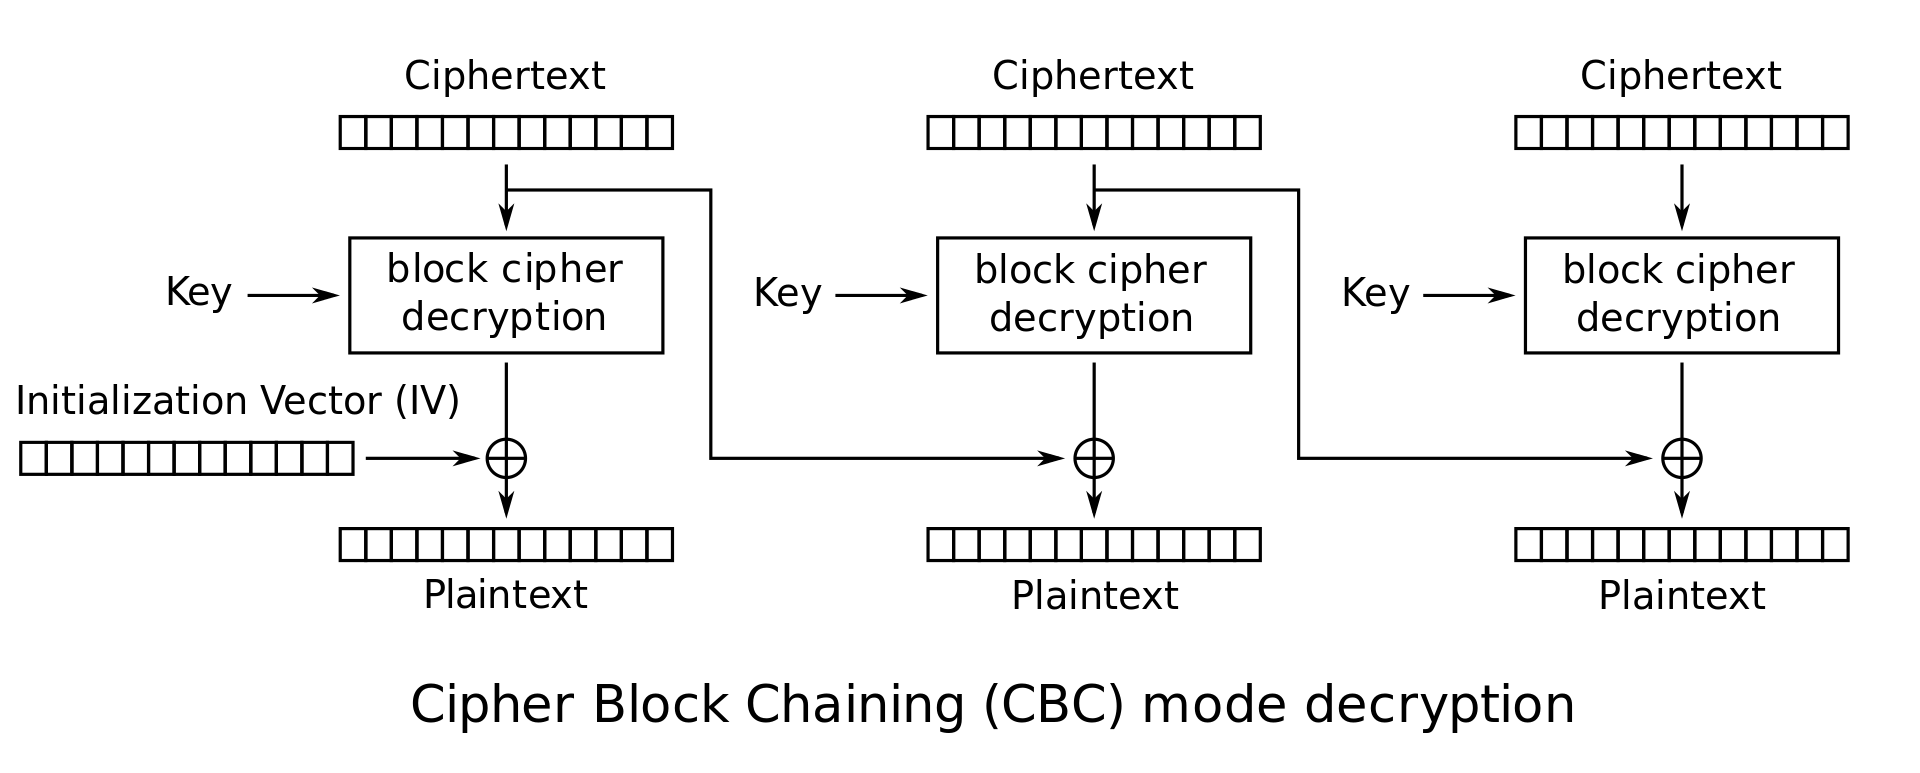
\includegraphics[width=12cm]{./Literatur/documents/CBC_decryption}\newline\caption{Entschlüsselung im CBC-Mode~\cite{CBC-entschluesseln}}
            \label{CBC_Mode_brechen}
        \end{center}
    \end{figure}


    \section{Sicherheitsbewertung}\label{sec:sicherheitsbewertung}
    Die Schwachstelle Lucky 13 wird allgemein mit einer geringen Sicherheitsbewertungsstufe angegeben~\cite{DATABASE2013}.
    Begründungen hierfür ist in erster Linie auch die Erkennung des richtigen Paddings.
    Das ist allerdings unwahrscheinlich, wenn man sich nicht im selben Netzwerk wie der Server befindet.
    Nadhem J. AlFardan and Kenneth G. Paterson haben die Analysen für ihr Paper auch nur im selben Netzwerk durchgeführt.
    \emph{SuSE} schreibt dazu ``Please note that an exploit for this requires physical proximity of an attacker to the server, which is usually unlikely``.
    Übersetzt bedeutet dies: Bitte beachten Sie, dass ein Exploit für dieses Problem die physische Nähe eines Angreifers zum Server erfordert, was in der Regel unwahrscheinlich ist.
    \newline
    Die Bewertung von Schwachstellen findet anhand des Common Vulnerability Scoring System (CVSS v2) statt.
    Dies ist der Industriestandard zur Bewertung für mögliche und tatsächliche Sicherheitslücken.
    Dort werden verschiedene Kategorien, die in~\ref{tab:CVSS-Vektor} zusehen sind, bewertet und dann nach einer Formel ein Wert zwischen 0 und 10 ermittelt.
    Je geringer der Wert ist, desto kleiner ist das Risiko.
    Auf der Skala ist das Risiko bis 3.9 gering, zwischen 4.0 und 6.9 ist es mittel und ab 7.0 ist das Risiko hoch.
    Deshalb wird von \emph{SuSE} der CVSS-Vector wie folgt gesetzt:
    \begin{table}[h]
        \begin{tabular}{lllll}
        {\ul \textbf{Exploitability Metrics}}
            &         & & {\ul \textbf{Impact Metrics}}   & \multicolumn{1}{c}{} \\
            \textbf{Access Vector}     & Network & & \textbf{Confidentiality Impact} & Partial              \\
            \textbf{Access Complexity} & High    & & \textbf{Integrity Impact}       & None                 \\
            \textbf{Authentication}    & None    & & \textbf{Availability Impact}    & None
        \end{tabular}\caption{Bewertung von Lucky 13 durch \emph{SuSE} in der CVSS-Skalar (Version 2) \cite{SuSE2013}}\label{tab:CVSS-Vektor}
    \end{table}
    \newline
    Das ergibt den Vektor AV:N/AC:H/Au:N/C:P/I:N/A:N mit einem CVSS-Score von 2.6.
    \emph{IBM} bewertet Lucky 13 gleich, außer in Hinsicht auf die Access Complexity, die als mittel gewertet wird, wodurch die Gesamtbewertung auf 4.3 ansteigt~\cite{IBM2013}.
    Die beiden Bewertungen fallen gering aus, die von \emph{SuSE} ist im niedrigen Risiko und die von \emph{IBM} im mittleren Bereich.
    Damit ist es unwahrscheinlich, Opfer durch den Lucky 13 Angriff zu werden.


    \section{Gegenmaßnahmen}\label{sec:gegenmanahmen}
    Es gibt mehrere Maßnahmen, die ergriffen werden können, um einen Angriffserfolg zu minimieren.
    Die Maßnahmen müssen verhindern, dass man eine Zeitanalyse durchführen kann oder sie muss das benötigte Padding in der Blockverschlüsslung umgehen.

    \subsection{Zufällige Zeitverzögerungen}\label{subsec:zufallige-zeitverzogerungen}
    Bei einem Angriff, der auf die Dauer einer Reaktion abzielt, liegt eine zufällige verzögerung nahe.
    Allerdings ist dies ineffektiv wie N. AlFardan und K. G. Paterson schreiben~\cite[S.13]{AlFardan2013}.

    \subsection{Rons's Code 4 Chiffre}\label{subsec:rons's-code-4-chiffre}
    Die Ron's Code 4 Chiffre (RC4) wird zum bei der Veröffentlichung von N. AlFardan und K. G. Paterson als eine Möglichkeit zum Schutz erwähnt, weil kein Padding benötigt wird.
    Allerdings wurde auch gesagt, dass dies keine Möglichkeit für DTLS ist~\cite[S.13]{AlFardan2013}.
    2015 wurde von der Internet Engineering Task Force (IETF)  die Nutzung und Kommunikation über RC4 in verbindung mit TLS verboten, weil es Sicherheitsmängel aufweist~\cite{IETF2015}.

    \subsection{Implementierung der MEE-TLS-CBC-Entschlüsselung}\label{subsec:implementierung-der-mee-tls-cbc-entschlusselung}
    Dies ist die von den Publishern des Angriffs empfohlene Methode.
    Dabei geht es darum, die Verarbeitungszeit nicht von dem Inhalt oder dem Padding abhängig zu machen, sondern nur von der Länge der chiffrierten Nachricht~\cite[S.13]{AlFardan2013}.
    Der größte Zeitunterschied entstehen bei der MAC Verarbeitung, weshalb da darauf geachtet werden muss.

    \newpage

    \bibliography{Literatur/Quellen}
\end{document}

